\renewcommand{\tvexists}[1]{\makebox{E($#1$) }}
\renewcommand{\tvforall}[1]{\makebox{A($#1$) }}
\renewcommand{\tvand}{\makebox{ $\&$ }}
\renewcommand{\tvor}{\makebox{ $|$ }}
\renewcommand{\tvstar}{\makebox{$*$}}
\renewcommand{\tvplus}{\makebox{$+$}}
\renewcommand{\tvneq}{\makebox{ $!=$ }}
\renewcommand{\tvneg}{\makebox{ $!$ }}
\renewcommand{\tveq}{\makebox{ $==$ }}

\begin{figure}
\framebox{
\begin{minipage}{1in}
\begin{tabbing}
// Set of names of program variables.\\
\tvset\ PVar\ \{x, y, t\}\\
/* Program variables definition */\\
\foreach\ \= (z \inset\ Var)  \{\+ \\
 \predicate\ $z(v1)$ unique pointer
 \- \\
\}\\
// A predicate to represent the n field of the list data type.\\
\predicate\ $n(v1, v2)$ function
\\
// Is shared instrumentation.\\
\instrum\ $is[n](v) = \tvexists{v1, v2} (v1 \tvneq v2 \tvand n(v1, v) \tvand n(v2, v))$\\
// Reachability instrumentation.\\
\foreach\ (z \inset\ PVar) \{
\instrum\ $r[n,z](v) =\tvexists{v1} (z(v1) \tvand n\tvstar(v1, v))$ \}\\
// The t[n] predicate records transitive reflexive reachability between\\
// list elements along the n field.\\
\instrum\ $t[n](v1, v2) = n*(v1, v2)$ transitive reflexive\\
// Cyclicity instrumentation.\\
\instrum\ $c[n](v) = n\tvplus(v, v)$
\end{tabbing}
\end{minipage}
}
\caption{\label{Fi:ManRevDecl}The declarations part of the TVP for the reverse
function shown in \figref{Reverse}.}
\end{figure}

\begin{figure}
\framebox{
\begin{minipage}{1in}
\begin{tabbing}
/******************************** Generic Actions *****************************/\\
\actionI\  Is\_Not\_Null\_Var(x1) \{
    \tvtitle\  x1 + " != NULL"\\
    \focus\  \{ $x1(v)$ \}
    \precond\  $\tvexists{v} x1(v)$\-\\
\}\\
\actionI\  Is\_Null\_Var(x1) \{
    \tvtitle\  x1 + " == NULL"\\
    \focus\  \{ $x1(v)$ \}
    \precond\  $\tvneg(\tvexists{v} x1(v))$\-\\
\}\\
/********************************* List Actions *******************************/\\
\actionI\  Set\_Null\_L(x1) \{
    \tvtitle\  x1 + " = NULL"\\
    \{  \= \+
        $x1(v) = 0$
%\\
%       $nn[x1]() = 0$\\
%        $r[n,x1](v) = 0$\-
    \}\-\\
\}\\
\actionI\  Copy\_Variable\_L(x1, x2) \{
    \tvtitle\  x1 + " = " + x2\\
    \focus\  \{ $x2(v)$ \}\\
    \{  \= \+
        $x1(v) = x2(v)$
  %  \\
 %       $nn[x1]() = nn[x2]()$\\
 %       $r[n,x1](v) = r[n,x2](v)$
 \-
    \}\-\\
\}\\
\actionI\  Get\_Next\_L(x1, x2) \{
    \tvtitle\  x1 + " = " + x2 + "\deref" + n\\
    \focus\  \{ $\tvexists{v1} x2(v1) \tvand n(v1, v)$\}\\
    \{  \= \+
        $x1(v) = \tvexists{v1} x2(v1) \tvand n(v1, v)$
%\\
 %       $nn[x1]() = \tvexists{v1, v} x2(v1) \tvand n(v1, v)$\\
 %       $r[n,x1](v) = r[n,x2](v) \tvand (c[n](v) \tvor \tvneg x2(v))$
 \-
    \}\-\\
\}\\
\actionI\  Set\_Next\_Null\_L(x1) \{
    \tvtitle\  x1 + "\deref" + n + " = NULL"\\
    \focus\  \{ $x1(v)$ \} \\
    \{  \= \+
        $n(v1, v2) = n(v1, v2) \tvand \tvneg x1(v1)$
    %\\
 %       $is[n](v) = is[n](v) \tvand ($\=$\tvneg(\tvexists{v1} x1(v1)
  %              \tvand n(v1, v)) \tvor$\\
  %           \>$\tvexists{v1, v2} v1 \tvneq v2 \tvand
  %           (n(v1, v) \tvand \tvneg x1(v1)) \tvand$\\
  %           \>$(n(v2, v) \tvand \tvneg x1(v2)))$\\
  %      $r[n,x1](v) = x1(v)$\\
  %      \foreachI(z in PVar-\{x1\}) \{\\
  %        $r[n,z](v) =$\=$ (c[n](v) \tvand r[n,x1](v) ?$\\
  %           \>$z(v) \tvor \tvexists{v1} z(v1) \tvand TC (v1, v) (v3, v4)
  %           (n(v3, v4) \tvand \tvneg x1(v3)) :$\\
  %           \>$r[n,z](v) \tvand \tvneg (r[n,x1](v) \tvand \tvneg x1(v) \tvand
  %              \tvexists{v1} r[n,z](v1) \tvand x1(v1)))$\-\\
  %      \}\\
  %      $c[n](v) = c[n](v) \tvand \tvneg (\tvexists{v1} x1(v1) \tvand
  %                 c[n](v1) \tvand r[n,x1](v))$
  \-
    \}\-\\
\}\\
\actionI\  Set\_Next\_L(x1, x2) \{
    \tvtitle\  x1 + "\deref" + n + " = " + x2\\
    \focus\  \{ $x1(v), x2(v)$ \}\\
    \{  \= \+
        $n(v1, v2) = n(v1, v2) \tvor x1(v1) \tvand x2(v2)$
  %      \\
  %      $is[n](v) = is[n](v) \tvor \tvexists{v1} x2(v) \tvand n(v1, v)$\\
  %      \foreachI(z in PVar) \{\\
  %        $r[n,z](v) = r[n,z](v) \tvor r[n,x2](v) \tvand \tvexists{v1} r[n,z](v1)
  %           \tvand x1(v1)$\-\\
  %      \}\\
  %      $c[n](v) = c[n](v) \tvor (r[n,x2](v) \tvand \tvexists{v1} x1(v1) \tvand
  %         r[n,x2](v1))$
  \-
    \}\-\\
\}
\end{tabbing}
\end{minipage}
}
\caption{\label{Fi:ManRevActions}The actions part of the TVP for the reverse
function shown in \figref{Reverse}.}
\end{figure}

\begin{figure}
\framebox{
\begin{minipage}{1.8in}
\begin{tabbing}
/* The program's CFG and the \= effect of its edges */\\
$L1$ Set\_Null\_L(y)         $L2$   \>// y = NULL;\\
$L2$ Is\_Null\_Var(x)        $exit$ \>// while (x != NULL) \{\\
$L3$ Is\_Not\_Null\_Var(x)   $L3$   \>//   x != NULL\\
$L3$ Copy\_Variable\_L(t, y) $L4$   \>//   t = y;\\
$L4$ Copy\_Variable\_L(y, x) $L5$   \>//   y = x;\\
$L5$ Get\_Next\_L(x, x)      $L6$   \>//   x = x\deref n;\\
$L6$ Set\_Next\_Null\_L(y)   $L7$   \>//   y\deref n = NULL;\\
$L7$ Set\_Next\_L(y, t)      $L8$   \>//   y\deref n = t;\\
$L8$ Set\_Null\_L(t)         $L2$   \>//   t = NULL;\\
                                    \>// \}\\
exit Assert\_ListInvariants(y) error\\
exit Assert\_No\_Leak(y) error
\end{tabbing}
\end{minipage}
}
\\
\begin{minipage}{1.8in}
\vspace{0.4cm}
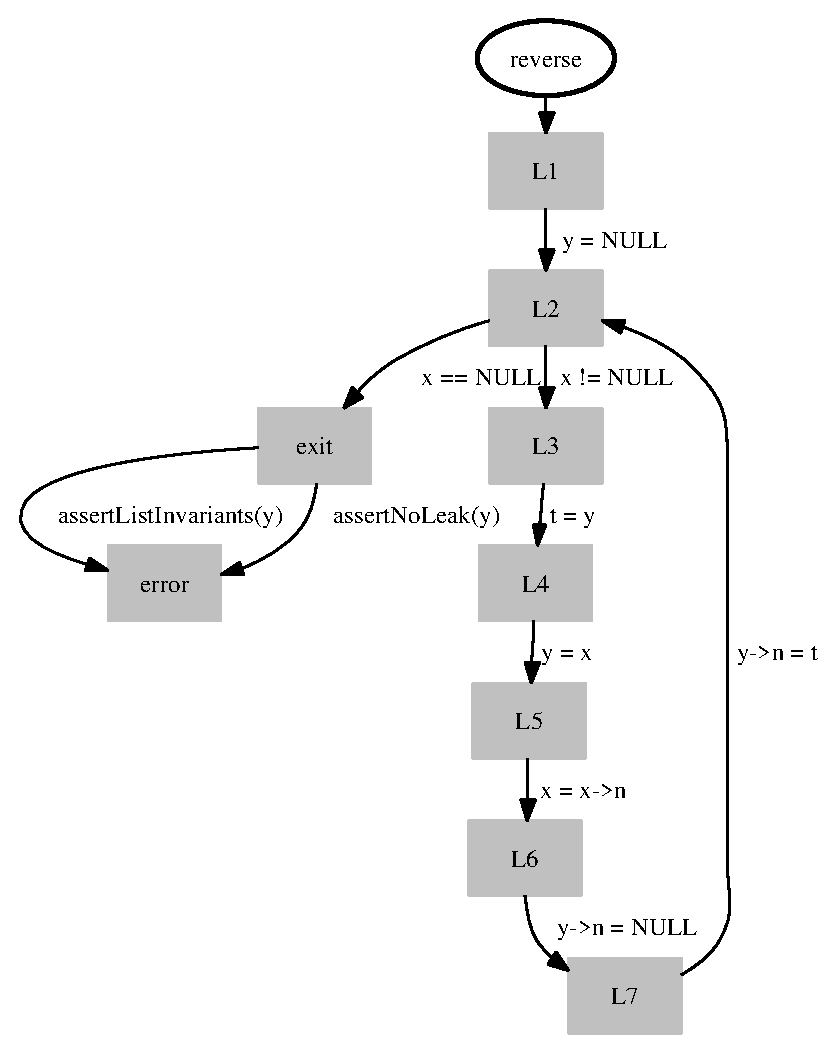
\epsfig{file=reverse_cfg,width=2.8in,height=3.0in}
\end{minipage}
\caption{\label{Fi:ManRevCFG}The CFG part of the TVP for the reverse function
shown in \figref{Reverse} and its corresponding CFG.}
\end{figure}
